\section{experiment}

To rigorously evaluate R\&D-Agent's capabilities in realistic data science scenarios, we conduct extensive experiments on MLE-Bench~\citep{chan2024mle-bench}. As a benchmark comprising a diverse set of authentic Kaggle competitions, MLE-Bench serves as an excellent proxy for real-world challenges, demanding a holistic combination of strategic thinking and robust engineering for agents to autonomously design, build, and train models.

\subsection{Experiment Setup}
\label{sec:exp_setup}
All our experiments are conducted on the MLE-Bench~\citep{chan2024mle-bench} benchmark. We compare R\&D-Agent against leading open-source systems, primarily ML-Master~\citep{liu2025ml} and AIDE~\citep{aide2025}, using their official leaderboard metrics. 
% Our experimental setup is intentionally more \textbf{challenging} than the standard setting: while the official setting allows for 24 hours, our agents operated under a stricter 12-hour time limit in an environment with 12 vCPUs, 220GB of RAM, and 1 V100 GPU.
In time budget, we align with ML-Master allowing 12 hours compared to the official 24 hours setting. In computation, our environment has a lower throughput with 12 vCPUs, 220GB RAM, and 1 V100 GPU while AIDE uses 36 vCPU, 440GB RAM and 1 A10 GPU, ML-Master uses 36 vCPU, 512GB shared  RAM and 1 A100 GPU. Therefore, our experimental setup is intentionally more \textbf{challenging} than all the previous work. 

To ensure fair comparison, we evaluate R\&D-Agent using two frontier LLM configurations: (1) GPT-5 only, and (2) a hybrid o3(R) + GPT-4.1(D), where o3 powers the Research phase and GPT-4.1 the Development phase. Furthermore, We re-evaluated the previous SOTA, ML-Master, under our identical 12-hour setting using both configurations. All our new results are averaged over three runs with different random seeds for statistical robustness. Our evaluation is based on the official MLE-Bench metrics, with the Any-Medal Rate as the primary indicator of overall performance.



% In this section, we demonstrate that R\&D-Agent achieves SOTA performance among fully automatic, open-source systems on this benchmark. Furthermore, through in-depth ablation studies, we validate the effectiveness of our core design components.



% \subsection{Experiment Setting}

% % \textbf{Configuration.} In the main experiment, the scheduler launches four exploration traces (with at most three running concurrently) and uses adaptive timeouts that start at 10 minutes for the Coder stage and 1 hour for the Runner stage, automatically extending to 40 minutes and 4 hours respectively whenever a stage exhausts its current limit.
% % % move to main exp





% \textbf{Hardware.} The environment we provided to R\&D-Agent and baseline systems includes 12 vCPUs, 220GB of RAM, and 1 V100 GPU, following the standard MLE-Bench~\citep{chan2024mle-bench} evaluation setting.

% \textbf{Metrics.} Our primary metric is the \emph{Any-Medal rate}\footnote{The percentage of benchmark tasks on which the agent secures at least a bronze medal.}. For ablation studies we additionally record (i) the number of optimization loops completed within the time budget, and (ii) the time-to-first-medal, namely the wall-clock time elapsed before the agent obtains its first qualifying submission.

% \textbf{Baselines.}  We establish comparisons with the leading open-source systems that currently achieve top rankings on the MLE-Bench~\citep{chan2024mle-bench} leaderboard, specifically ML-Master~\citep{liu2025ml} and AIDE~\citep{aide2025}.

% \textbf{Backend LLMs.} The R\&D Agent is compatible with various advanced LLMs. In the experiments, we utilize the following models: GPT-5, o3, GPT-4.1.The appendix contains a comprehensive analysis of experimental outcomes obtained using various LLM combinations for the coder and runner components.





% \begin{table}[!t]
% \centering
% \caption{Performance comparison on MLE-Bench~\citep{chan2024mle-bench}. Best results in each column are in \textbf{bold}.}
% \label{tab:performance}
% \small
% \begin{tabularx}{\textwidth}{lYYYY}
% \toprule
% \textbf{Agent} & \textbf{Low==Lite(\%)} & \textbf{Medium(\%)} & \textbf{High(\%)} & \textbf{All(\%)} \\
% \midrule
% \multicolumn{5}{l}{\textbf{MLAB~\cite{huang2023mlagentbench}}} \\
% \midrule
% GPT-4o & 4.2 \,$\pm$\, 1.5 & 0.0 \,$\pm$\, 0.0 & 0.0 \,$\pm$\, 0.0 & 1.3 \,$\pm$\, 0.5\\
% \midrule
% \multicolumn{5}{l}{\textbf{OpenHands~\cite{wang2024openhands}}} \\
% \midrule
% GPT-4o & 11.5 \,$\pm$\, 3.4 & 2.2 \,$\pm$\, 1.3 & 1.9 \,$\pm$\, 1.9 & 5.1 \,$\pm$\, 1.3\\
% \midrule
% \multicolumn{5}{l}{\textbf{AIDE~\cite{aide2025}}} \\
% \midrule
% GPT-4o & 19.0 \,$\pm$\, 1.3 & 3.2 \,$\pm$\, 0.5 & 5.6 \,$\pm$\, 1.0 & 8.6 \,$\pm$\, 0.5\\
% o1-preview & 34.3 \,$\pm$\, 2.4 & 8.8 \,$\pm$\, 1.1 & 10.0 \,$\pm$\, 1.9 & 16.9 \,$\pm$\, 1.1 \\
% \midrule
% \multicolumn{5}{l}{\textbf{ML-Master~\cite{liu2025ml}}} \\
% \midrule
% Deepseek-R1 & 48.5 \,$\pm$\, 1.5 & 20.2 \,$\pm$\, 2.3 & 24.4 \,$\pm$\, 2.2 & 29.3 \,$\pm$\, 0.8 \\
% GPT-5 & & & & \\
% \midrule
% \multicolumn{5}{l}{\textbf{R\&D-Agent (Ours)}} \\
% \midrule
% GPT-5 & \textbf{68.2 \,$\pm$\,2.6} & \textbf{21.1\,$\pm$\,1.5} & 22.2 \,$\pm$\,2.2 & \textbf{35.1\,$\pm$\,0.4}\\
% \bottomrule
% \end{tabularx}
% \end{table}

% For the main experimental setup, we configured a concurrency limit of 4 traces with parallel execution capped at 3 simultaneous traces. We implemented adaptive timeout mechanisms, with initial timeout periods of 10 minutes for the Coder stage and 1 hour for the Runner stage. These timeouts automatically extend to 40 minutes and 4 hours, respectively, when a stage reaches its current time limit.

\subsection{Main Results}

R\&D-Agent establishes a new SOTA on MLE-Bench~\citep{chan2024mle-bench}, significantly outperforming all existing open-source systems. As illustrated in Figure~\ref{fig:agent_result}, R\&D-Agent powered by GPT-5 achieves 35.1\% Any-Medal Rate, exceeding the previous state-of-the-art ML-Master~\citep{liu2025ml} (29.3\% with Deepseek-R1) by 5.8 percentage points. The stacked bars further reveal R\&D-Agent's consistent superiority across all task complexity levels, demonstrating its robust performance on diverse data science challenges.

Table~\ref{tab:full-results} further demonstrates our framework's architectural advantages. With GPT-5, R\&D-Agent achieves the highest Any-Medal Rate at 35.1 \,$\pm$\,0.4\%, while our hybrid o3(R) + GPT-4.1(D) configuration also excels at 29.7 \,$\pm$\,0.4\%, with both substantially outperforming all prior systems. Crucially, when ML-Master was re-evaluated with GPT-5 in our environment, it achieved only 16.9 \,$\pm$\,2.0\%\footnote{This differs from ML-Master's official 29.3\% primarily due to: (1) hardware differences (V100 vs. A100 GPU), and (2) backend model differences (GPT-5 vs. Deepseek-R1). We report this for transparent comparison under identical conditions.}. This direct comparison under identical LLM configurations confirms that our framework's design, not merely model selection, drives the substantial performance gap. Both R\&D-Agent configurations demonstrate strong performance across multiple metrics, with GPT-5 achieving 45.3 \,$\pm$\,0.0\% Above-Median Rate and 16.4 \,$\pm$\,0.9\% Gold Medal Rate, showcasing the framework's ability to consistently produce competitive solutions regardless of the underlying LLM choice.


% \begin{table}[!h]
% \centering
% \caption{Comparative performance of all agents across the official MLE-Bench evaluation metrics. All results represent the mean \,$\pm$\,SEM from three independent runs with different random seeds. The top-performing agent is highlighted in \textbf{bold} and the second-best is \underline{underlined}. * indicates our re-evaluation of ML-Master~\citep{liu2025ml} within our environment (V100 GPU) to ensure fair comparison under identical conditions. Complete individual run results are provided in Appendix~\ref{sec:main_results_details}.}
% \label{tab:full-results}
% \small
% % \begin{tabularx}{\textwidth}{lYYYYYY}
% \begin{tabular}{l c c c c c >{\columncolor{gray!10}}p{1.4cm}}
% \toprule
% \textbf{Agent}  &
% \makecell{\textbf{Valid} \\ \textbf{Submission} \\ \textbf{(\%)} } &
% \makecell{\textbf{Above} \\ \textbf{Median} \\ \textbf{(\%)} } &
% \makecell{\textbf{Bronze} \\ \textbf{(\%)} } &
% \makecell{\textbf{Silver} \\ \textbf{(\%)} } &
% \makecell{\textbf{Gold} \\ \textbf{(\%)} } &
% \makecell{\textbf{Any} \\ \textbf{Medal} \\ \textbf{(\%)} } \\
% \midrule

% \multicolumn{7}{l}{\textbf{MLAB~\citep{huang2023mlagentbench}}} \\
% \midrule
% GPT-4o & 44.3 \,$\pm$\,2.6 & 1.9 \,$\pm$\,0.7 & 0.0 \,$\pm$\,0.0 & 0.0 \,$\pm$\,0.0 & 0.8 \,$\pm$\,0.5 & 0.8 \,$\pm$\,0.5\\
% \midrule
% \multicolumn{7}{l}{\textbf{OpenHands~\citep{wang2024openhands}}} \\
% \midrule
% GPT-4o & 52.0 \,$\pm$\,3.3 & 7.1 \,$\pm$\,1.7 & 0.4 \,$\pm$\,0.4 & 1.3 \,$\pm$\,0.8 & 2.7 \,$\pm$\,1.1 & 4.4 \,$\pm$\,1.4\\
% \midrule
% \multicolumn{7}{l}{\textbf{AIDE~\citep{aide2025}}} \\
% \midrule
% GPT-4o & 54.9 \,$\pm$\,1.0 & 14.4 \,$\pm$\,0.7 & 1.6 \,$\pm$\,0.2 & 2.2 \,$\pm$\,0.3 & 5.0 \,$\pm$\,0.4 & 8.7 \,$\pm$\,0.5\\
% o1-preview & 82.8 \,$\pm$\,1.1 & 29.4 \,$\pm$\,1.3 & 3.4 \,$\pm$\,0.5 & 4.1 \,$\pm$\,0.6 & 9.4 \,$\pm$\,0.8 & 16.9 \,$\pm$\,1.1\\
% \midrule
% \multicolumn{7}{l}{\textbf{ML-Master~\citep{liu2025ml}}} \\
% \midrule
% Deepseek-R1 & 93.3 \,$\pm$\,1.3 & \underline{44.9 \,$\pm$\,1.2} & 4.4 \,$\pm$\,0.9 & \underline{7.6 \,$\pm$\,0.4} & \textbf{17.3 \,$\pm$\,0.8} & 29.3 \,$\pm$\,0.8 \\
% % Deepseek-R1(R) & 92 \,$\pm$\,1.3 & 36.9 \,$\pm$\,2 & 4.4 \,$\pm$\,0.8 & 4.4 \,$\pm$\,0.8 & 13.8 \,$\pm$\,1.5 & 22.7 \,$\pm$\,1.3 \\
% o3(R) + GPT-4.1(D)* & \textbf{98.2 \,$\pm$\,0.9} & 25.8 \,$\pm$\,1.9 &5.8 \,$\pm$\,1.6 &3.1 \,$\pm$\,1.9 &9.3 \,$\pm$\,0.8 & 18.2 \,$\pm$\,1.9 \\
% GPT-5* & 85.3 \,$\pm$\,3.5 &26.2 \,$\pm$\,1.6 &4.4 \,$\pm$\,1.2&3.1 \,$\pm$\,0.4 &9.3 \,$\pm$\,0.8 & 16.9 \,$\pm$\,1.2\\
% \midrule
% \multicolumn{7}{l}{\textbf{R\&D-Agent (Ours)}} \\
% \midrule
% o3(R) + GPT-4.1(D) & 94.2 \,$\pm$\,0.4 & \underline{44.9 \,$\pm$\,0.4} & \underline{6.2 \,$\pm$\,0.9} & 7.5 \,$\pm$\,1.2 & 16.0 \,$\pm$\,0.8 & \underline{29.7 \,$\pm$\,0.4} \\
% GPT-5 & \underline{96.0 \,$\pm$\,0.0}  & \textbf{45.3 \,$\pm$\,0.0} & \textbf{6.7 \,$\pm$\,1.5} & \textbf{12.0 \,$\pm$\,0.8} & \underline{16.4 \,$\pm$\,0.9} & \textbf{35.1 \,$\pm$\,0.4} \\
% \bottomrule
% \end{tabular}
% \end{table}

\begin{table}[!h]
\centering
\caption{Comparative performance of all agents across the official MLE-Bench evaluation metrics. All results represent the mean $\pm$ SEM from three independent runs with different random seeds. The top-performing agent is highlighted in \textbf{bold} and the second-best is \underline{underlined}. * indicates our re-evaluation of ML-Master~\citep{liu2025ml} within our environment (V100 GPU) to ensure fair comparison under identical conditions. Complete individual run results are provided in Appendix~\ref{sec:main_results_details}.}
\label{tab:full-results}
\small
\setlength{\tabcolsep}{5pt}
\begin{tabular}{l c c c c c >{\columncolor{gray!10}}p{1.4cm}}
\toprule
\textbf{Agent} &
\makecell{\textbf{Valid}\\\textbf{Submission}\\\textbf{(\%)}} &
\makecell{\textbf{Above}\\\textbf{Median}\\\textbf{(\%)}} &
\makecell{\textbf{Bronze}\\\textbf{(\%)}} &
\makecell{\textbf{Silver}\\\textbf{(\%)}} &
\makecell{\textbf{Gold}\\\textbf{(\%)}} &
\makecell{\textbf{Any}\\\textbf{Medal}\\\textbf{(\%)}} \\
\midrule

\multicolumn{7}{l}{\textbf{MLAB~\citep{huang2023mlagentbench}}} \\
\midrule
GPT-4o & $44.3 \pm 2.6$ & $1.9 \pm 0.7$ & $0.0 \pm 0.0$ & $0.0 \pm 0.0$ & $0.8 \pm 0.5$ & $0.8 \pm 0.5$ \\
\midrule

\multicolumn{7}{l}{\textbf{OpenHands~\citep{wang2024openhands}}} \\
\midrule
GPT-4o & $52.0 \pm 3.3$ & $7.1 \pm 1.7$ & $0.4 \pm 0.4$ & $1.3 \pm 0.8$ & $2.7 \pm 1.1$ & $4.4 \pm 1.4$ \\
\midrule

\multicolumn{7}{l}{\textbf{AIDE~\citep{aide2025}}} \\
\midrule
GPT-4o       & $54.9 \pm 1.0$ & $14.4 \pm 0.7$ & $1.6 \pm 0.2$ & $2.2 \pm 0.3$ & $5.0 \pm 0.4$ & $8.7 \pm 0.5$ \\
o1-preview   & $82.8 \pm 1.1$ & $29.4 \pm 1.3$ & $3.4 \pm 0.5$ & $4.1 \pm 0.6$ & $9.4 \pm 0.8$ & $16.9 \pm 1.1$ \\
\midrule

\multicolumn{7}{l}{\textbf{ML-Master~\citep{liu2025ml}}} \\
\midrule
Deepseek-R1                  & $93.3 \pm 1.3$ & \underline{$44.9 \pm 1.2$} & $4.4 \pm 0.9$ & \underline{$7.6 \pm 0.4$} & $\mathbf{17.3 \pm 0.8}$ & $29.3 \pm 0.8$ \\
% Deepseek-R1(R)             & $92.0 \pm 1.3$ & $36.9 \pm 2.0$ & $4.4 \pm 0.8$ & $4.4 \pm 0.8$ & $13.8 \pm 1.5$ & $22.7 \pm 1.3$ \\
o3(R) + GPT-4.1(D)*          & $\mathbf{98.2 \pm 0.9}$ & $25.8 \pm 1.9$ & $5.8 \pm 1.6$ & $3.1 \pm 1.9$ & $9.3 \pm 0.8$ & $18.2 \pm 1.9$ \\
GPT-5*                       & $85.3 \pm 3.5$ & $26.2 \pm 1.6$ & $4.4 \pm 1.2$ & $3.1 \pm 0.4$ & $9.3 \pm 0.8$ & $16.9 \pm 1.2$ \\
\midrule

\multicolumn{7}{l}{\textbf{R\&D-Agent (Ours)}} \\
\midrule
o3(R) + GPT-4.1(D)           & $94.2 \pm 0.4$ & \underline{$44.9 \pm 0.4$} & \underline{$6.2 \pm 0.9$} & $7.5 \pm 1.2$ & $16.0 \pm 0.8$ & \underline{$29.7 \pm 0.4$} \\
GPT-5                        & \underline{$96.0 \pm 0.0$} & $\mathbf{45.3 \pm 0.0}$ & $\mathbf{6.7 \pm 1.5}$ & $\mathbf{12.0 \pm 0.8}$ & \underline{$16.4 \pm 0.9$} & $\mathbf{35.1 \pm 0.4}$ \\
\bottomrule
\end{tabular}
\end{table}



\subsection{Ablation Study}
\label{sec:ablation}
We quantify each component's contribution by removing one component at a time while preserving all others. For computational efficiency, evaluations are conducted on a curated subset of 40 competitions from MLE-Bench~\citep{chan2024mle-bench} using GPT-5 (see Appendix~\ref{sec:competition_subset}). This subset includes tasks where our method, AIDE~\citep{aide2025}, or ML-Master~\citep{liu2025ml} achieved medals, ensuring coverage of scenarios most influenced by our design.

Our analysis aligns with the dual-phase architecture: the \textbf{research phase ablation} evaluates four components (\textit{dynamic planning}, \textit{exploration path structuring}, \textit{memory context}, and \textit{reasoning pipeline}), while the \textbf{development phase ablation} focuses on implementation elements (\textit{coding workflows} and \textit{evaluation strategy}).

\subsubsection{Research Phase Ablation Study}

Table \ref{tab:research-ablation} summarizes our analysis across four key metrics:
(1) \textbf{Avg. Loops}: number of R\&D loops per competition,
(2) \textbf{Improve Rate}: percentage of R\&D loops yielding performance gains,
(3) \textbf{First-Medal}: time to first medal-winning solution,
(4) \textbf{Medal Rate}: percentage achieving medals in the 40-competition subset.
(5) \textbf{Any Medal}: percentage achieving medals in the whole 75-competition set. The 35 remaining competitions are all considered non-medal in this calculation.
% , and
% \ding{196} \textbf{IC} (Spearman correlation between validation and test scores). \todo{I think we do not need the same number notation in methods here}
% \todo{IC is never used in this section.}
\begin{table}[ht]
    \caption{Research Phase Ablation Results on 40-competition subset. Each column removes one component while preserving others. Full System shows mean \,$\pm$\,SEM over 3 runs; ablation results report single representative runs due to computational constraints.}
    \label{tab:research-ablation}
    \renewcommand{\arraystretch}{1.2}
    \begin{center}
        \begin{minipage}{\linewidth}
        \setlength{\tabcolsep}{2.5pt}
            \begin{tabular}{lcccccc}
                \hline
                \textbf{Metric} & \textbf{Full System} & \textbf{w/o Planning} & \textbf{w/o Exploration} & \textbf{w/o Reasoning} & \textbf{w/o Memory}\\
                & & & \textbf{Path} & \textbf{Pipeline} & \textbf{Context}\\
                \hline
                Avg. Loops & 45.9 $\pm$ 2.2 & 48.4 & 19.4 & 55.3 & 44.0\\
                Improve Rate (\%) & 41.1 $\pm$ 0.4 & 39.4 & 40.0 & 23.0 & 40.9\\
                First-Medal (h) & 2.9 $\pm$ 0.1 & 1.7 & 3.0 & 1.7 & 2.0\\
                % First-Medal\_2 (h) & 5.6 $\pm$ 0.1 & 6.6 $\pm$ 0.3 & 5.3 $\pm$ 0.2 & 7.3 $\pm$ 0.4 & 6.4 $\pm$ 0.3\\
                % IC & 0.786 $\pm$ 0.014 & 0.734 & 0.677 & 0.728 & 0.783\\
                % % test 和 valid score的差异
                Medal Rate (\%) & 65.8 $\pm$ 0.8 & 50.0 & 47.5 & 50.0 & 60.0\\
                Any Medal (\%) & 35.1 $\pm$ 0.4 & 26.7 & 25.3 & 26.7 & 32\\
                \hline
            \end{tabular}
        \end{minipage}
    \end{center}
\end{table}
 
\vspace{-10pt}  

Each ablation reveals how R\&D-Agent degrades toward existing baselines (Table~\ref{tab:agent_comparison}), confirming our framework's architectural advantages:

\begin{itemize}[leftmargin=4ex, itemsep=0pt]

\item \textbf{w/o Planning (24\% relative decline).} Degrading component \textit{Planning} from \textit{Dynamic} to baseline approaches lacking strategic resource allocation ("/"). Any Medal Rate drops from 35.1\% to 26.7\%. Despite faster First-Medal time (2.9h$\rightarrow$1.7h), the system rushes to local optima without temporal adaptation, matching the performance degradation observed in methods like AIDE.

\item \textbf{w/o Exploration Path (28\% relative decline).} The most severe degradation occurs when degrading \textit{Adaptive} path structuring to sequential chain exploration (similar to MLE-STAR~\citep{nam2025mle}). Any Medal Rate drops to 25.3\% and average loops fall dramatically (45.9$\rightarrow$19.4), demonstrating how tree-based adaptive exploration fundamentally outperforms rigid chain structures in solution space coverage.

\item \textbf{w/o Reasoning Pipeline (24\% relative decline).} Degrading our \textit{Scientific multi-step} reasoning to baseline \textit{one-step} approaches used by prior methods. Any Medal Rate drops to 26.7\% and Improve Rate collapses (41.1\%$\rightarrow$23.0\%). Despite high exploration volume (55.3 loops), the system generates improvements in only 23\% of loops, highlighting how structured multi-step reasoning enables more effective hypothesis generation than simple one-step approaches.

\item \textbf{w/o Memory Context (9\% relative decline).} Degrading component \textit{Memory Context} from \textit{Collaborative Communication} to a simple memory management approach(similar to ML-Master~\citep{liu2025ml}), showing the smallest degradation to 32.0\% Any Medal Rate. The preserved iteration efficiency suggests that while collaborative memory provides optimization benefits, core learning mechanisms remain functional through alternative pathways, validating our architectural separation between fundamental and enhancement components.
\end{itemize}

These results demonstrate that R\&D-Agent's superior performance stems from architectural innovations, with exploration path structuring providing the most critical advantage over existing approaches. 

% \todo{I don't think emphasis this is meaningful} 
% The synergistic effects of these components collectively enable the sophisticated research capabilities that distinguish R\&D-Agent from simpler agent architectures.


\subsubsection{Development Phase Ablation Study}

Unlike research components that affect idea generation, development components impact solution implementation quality and reliability. We analyze their contributions through temporal medal acquisition patterns over 12 hours, as shown in Figure \ref{fig:development-ablation}. This temporal approach reveals not just final performance, but also \textit{when} and \textit{how quickly} each component contributes to success. Results combine ablation studies with one representative run from the primary experiment, illustrating the temporal dynamics of development components.

% Figure \ref{fig:development-ablation} shows cumulative medal counts over time for three configurations plus a theoretical upper bound.

\textbf{Perfect Selection (Upper Bound).} Theoretical maximum performance if we could submit all generated solutions and select the best performer. This oracle bound reaches 37.3\% Any Medal Rate, establishing our solution pool's upper limit.

\textbf{Full System.} Exhibits rapid initial progress (0-2h), steady refinement (2-6h), and convergence at 34.7\% Any Medal Rate. Achieving 93\% of perfect selection demonstrates effective solution identification without test set access.

\begin{wrapfigure}{r}{0.45\textwidth}
    \vspace{-20pt}
    \centering
    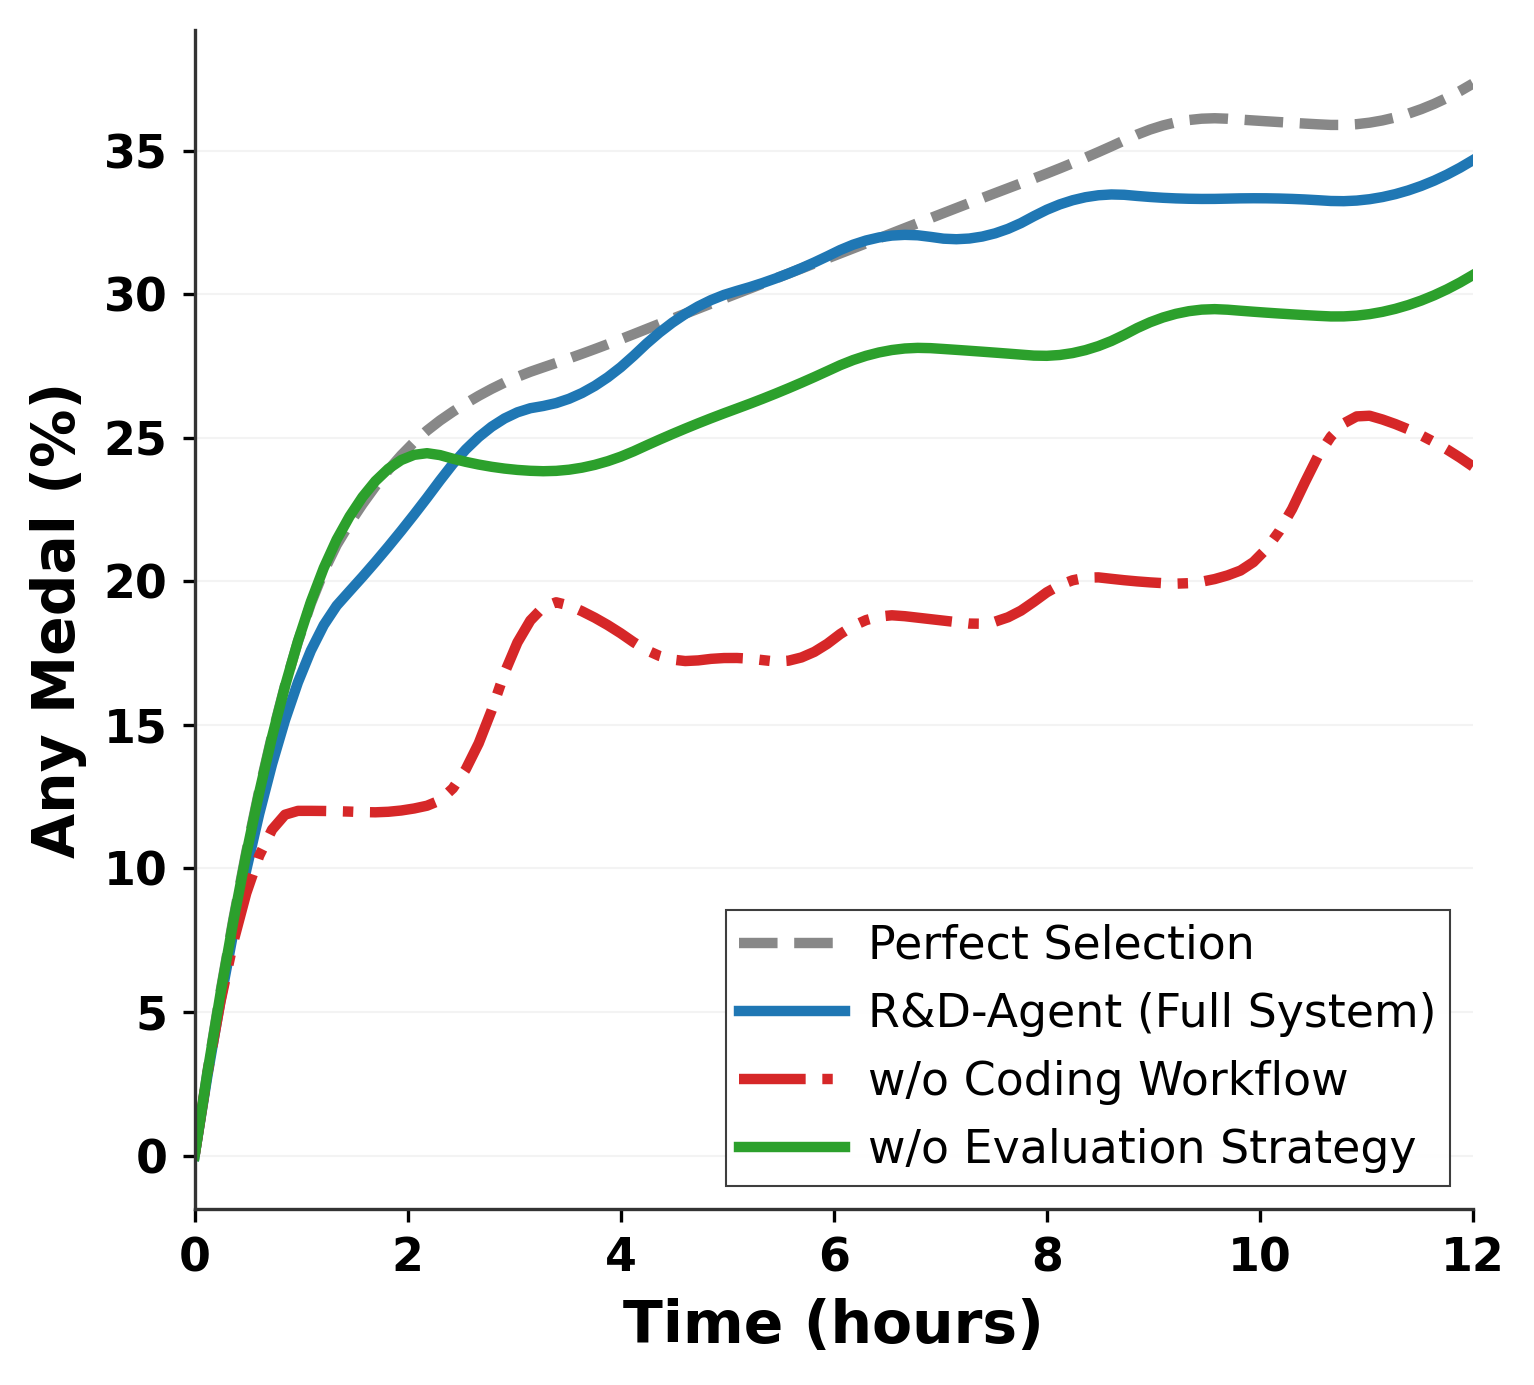
\includegraphics[width=0.43\textwidth]{Figures/development_ablation_narrow.png}
    \caption{Development Phase Temporal Ablation. Medal acquisition rate (percentage of 75 competitions) over 12 hours reveals when and how each component contributes.}
    \label{fig:development-ablation}
    \vspace{-25pt}
\end{wrapfigure}

\textbf{W/o Coding Workflow.} Degrading our \textit{Efficient \& Iterative Debug} workflow forces the system to use full-dataset debugging like baseline methods. Performance drops immediately to 24.0\% Any Medal Rate and remains persistently degraded. This demonstrates that our sample-based debugging fundamentally outperforms traditional full-dataset approaches, where computational overhead severely constrains exploration within time budgets—the same bottleneck that limits existing systems.

\textbf{W/o Evaluation Strategy.} Degrading our \textit{Aggregated} evaluation strategy to baseline approaches without systematic evaluation. Performance initially matches the full system until hour 2, then diverges significantly to 30.7\% Any Medal Rate. This delayed degradation shows that while basic evaluation suffices for simple solutions, sophisticated multi-dimensional evaluation becomes critical as solution complexity and over-fit risk increases-an advantage absent in existing methods.

These temporal patterns show how R\&D-Agent's development innovations address fundamental bottlenecks overlooked by prior work: coding workflow provides implementation efficiency from the start, while evaluation strategy enables sustained improvement as solutions grow sophisticated.


